\subsubsection{Protein Engineering}
\index{Schwaneberg, Ulrich}

\paragraph{Research Team}
%
Ulrich Schwaneberg (Professor), Alexander Schenk (Postdoc), Radivoje Prodanovic (Postdoc), Li-qing Zhao (Postdoc), Jovana Grujic (PhD Student), Josefa Caballero Hern�ndez (PhD Student), Carmen Momeu (PhD Student), Tuck Seng Wong (PhD Student), Kang Lan Tee (PhD Student), Ozana Onaca (PhD Student), Saskia Ihle (PhD Student), Milan Blanusa (PhD Student), Daniela Josuttis (BTA), Marina Linow (Head of Biotechnikum), Dr. Birgit Orthen (Associated, Head of BioHanse Bremen)\\


We are experts in biocatalyst engineering with a focus on directed
protein evolution. The core competence comprises the development
of novel methods for generating diversity on the gene level
(SeSaM: \cite{Schwaneberg8} \& \cite{Schwaneberg9} and novel high-throughput screening systems (\cite{Schwaneberg3}, \cite{Schwaneberg5} \&
\cite{Schwaneberg7}). SeSaM method is complemented by a statistical method named MAP
(Mutagenesis Assistant Program) to provide protein engineers for
the first time with a tool to benchmark current random mutagenesis
methods by investigating the consequences of mutational bias on
the protein level. Based on these core competences we collaborate
with companies (e.g. BASF AG, BRAIN AG, Henkel KGaA, Schering AG,
Degussa AG) and research groups (mainly in Bremen, Hamburg, Basel
and Austin (USA)). In these collaborations we apply our developed
technologies to solve significant problems in industrial
biocatalysis and to understand structure-function relationships of
biocatalysts.



\paragraph{Highlights}
%
2006 was the year in which we published our first articles in the
Miniature Biofuel Cell and Nanocompartment area. These now
established research fields open novel and innovative directions
for our future research activities (see Figure). Highlights in
2006 comprise: a) publication of 12 manuscripts in peer-reviewed
journals including one cover page in JMB; four manuscripts have
been published with colleagues at Jacobs University (Dr. Roccatano, Prof.
Zacharias, Prof. Winterhalter), b) successful establishment of the
SeSaM Profit Center for commercial exploitation of the
SeSaM-mutagenesis technology. A lighthouse project for the company
BRAIN AG was successfully completed in 2006, an evolved
biocatalyst is in the upscale process at BASF AG, and the
SeSaM-Biotech company will become operational in October 2007, c)
additional secrecy agreements have been signed with Henkel KGaA,
Degussa AG and BRAIN AG to exploit the SeSaM-Technology, d) a 430
T Euro award from the BMBF has been granted for pushing screening
technologies, e) a DFG workshop for the SPP1170 ``Gelenkte
Evolution'' has been organized on Jacobs University campus, and f) a BioHanse
Bremen competence center for coordinating academic biotechnology
activities in Bremen  was established with the ``Gesch�ftsstelle''
at Jacobs University (200 T Euro award; State of Bremen).

\begin{figure}[ht]
  \begin{center}
    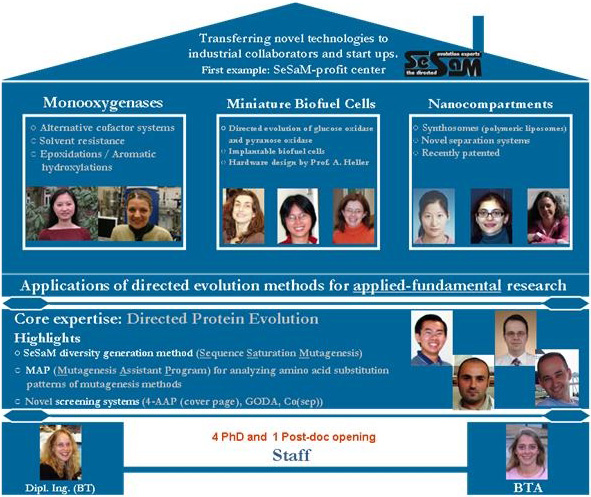
\includegraphics[width=\hsize]{Schwaneberg/Schwaneberg_2006_fig.png}
     \mycaption{Schwaneberg Research Group.}
  \end{center}
\end{figure}


\paragraph{Grants}
\begin{enumerate}
\item   Funded by ESF-COST, \emph{COST-D25-Biooxidation},
(November 2003   - October 2006)
 \item   Funded by BASF,  \emph{Esterase" und "Protease}, (April
2005  - March 2006)
 \item   Funded by DFG,
\emph{SeSaM, Sequence Saturation Mutagenesis and its application
in bioelectrocatalysis}, (September 2004  - August 2006)
 \item Funded by DBU, \emph{ICBio, Hochselektive
Bioaktivierung von Plattform-Intermediaten: Molekulares Screening,
funktionale �berexpression und umweltfreundliche elektrochemische
Verfahren}, (July 2004   -   June 2006)
 \item   Funded by SfBW - SfBUV, \emph{Selektive Isolierung von DNA und RNA in
Nanokontainern},  (January 2005    -   December 2007)
 \item
Funded by SfBW,  \emph{Bio-Hanse Bremen - Einrichtung eines
Kompetenzzentrums f�r Biotechnologie  }, (November 2005 - October
2007)
 \item Funded by DFG. \emph{Schw-2 Iterative
cycles, Understanding mediated/direct electron transfer and
solvent resistance by iterative cycles of directed monooxygenase
evolution and refinement of computational models },
(September 2006  -   August 2008)
 \item   Funded by BMBF,  \emph{BioChancePlus-BRAIN, Universelle
Hochdurchsatzdurchmusterungssystemen zum Auffinden industriell
bedeutsamer Biokatalysatoren in Metagenom-und
Zufallsmutagenese-Bibliotheken }, ( October 2006 - September 2009)

\item Funded by ONR, \emph{Making Glucose Oxidizing Enzymes Fit
for Biofuel Cell Applications}, (October 2002 - May 2006)
\end{enumerate}


\paragraph{Organization}
\begin{enumerate}
\item {Member of the Directorate and cofounder of the competence
center BioHanse Bremen and Bremen School of Biotechnology}
\item {Establishment of the SeSaM-profit center for exploiting the
economic potential of the SeSaM technology}
\end{enumerate}


\paragraph{Patents}

Two patents based on research at IUB. Eight patents in total (five
in collaboration with BASF AG)


\paragraph{Collaborations}
We are open to use our core competence in directed protein
evolution to study interesting structure-function relationships in
collaborative research effort with colleagues. An example is the
collaboration with the computational group of Prof. Zacharias/Dr.
Roccatano (four joint manuscripts), who provides and develops for
our evolved monooxygenase mutants (improved organic solvent
resistance, changes substrate specificity) rational design tools
and assists in statistical analysis of random mutagenesis mutants.
A further example is the nanocompartment system, which comprises
the collaborative work with two polymer chemists (Prof. Meier, who
moved from Jacobs University to Uni Basel; Stephan F\"{o}rster, Uni Hamburg) and
with Prof. Winterhalter (Professor for Biophysics), who probes the
compound flux through the channel proteins (1 joint publication).
We further collaborate with Prof. Wilmanns (DESY, EMBL, Hamburg;
one joint manuscript submitted) and various colleagues at Uni
Bremen (e.g. Prof. Jastorff, one manuscript in preparation),
Hochschule Bremen and Hochschule Bremerhaven. We have further
established collaborative projects or submitted joint grant
applications with Prof. Sun (Wuxi, China), Prof. Ma Yanhe
(Beijing, China), Prof. Socaciou (Rumania), Prof. Janssen
(The Netherlands), and Prof. Jankov (Serbia).


%\myparagraph{Collaborations}
%
%Bremen Area Collaborations:
%\begin{enumerate}
%\item {\sl Jacobs University Bremen} \\ Prof. F.O. Gl�ckner \\ Sulfatases
%\item {\sl Jacobs University Bremen}\\Prof. M. Zacharias and Dr. D. Roccatano \\Influence of Organic Cosolvents on the Industrially Important Enzyme P450 BM-3
%\end{enumerate}
%National \& International Collaborations:
%\begin{enumerate}
%\item{}
%\end{enumerate}

\nocite{Schwaneberg1,Schwaneberg2,Schwaneberg3,Schwaneberg4,Schwaneberg5,Schwaneberg6,Schwaneberg7,Schwaneberg8,Schwaneberg9,Schwaneberg10,Schwaneberg11,Schwaneberg12}
